\documentclass{sig-alt-release2}
\usepackage{url}
\usepackage{color}
\usepackage{graphics,graphicx}

\usepackage{epsfig}
\usepackage{epstopdf}

\usepackage{colortbl}
\usepackage{multirow}
\usepackage{booktabs}
\usepackage{ifthen}

\begin{document}
\newcommand{\todo}[1]{\textcolor{red}{#1}}
\def\newblock{\hskip .11em plus .33em minus .07em}

\conferenceinfo{DIM3} {2013, Glasgow, UK} 
\CopyrightYear{2013}
\clubpenalty=10000
\widowpenalty = 10000

\title{{Berserker Chat: Specification, Design and Implementation Report}}

\numberofauthors{1}
\author{
\alignauthor Dan Tomosoiu, Tony Lau, Hector Grebbell\\
\affaddr{Berserker}\\
\affaddr{DIM3}\\
\affaddr{Student numbers}\\
\email{\{1102486T, 1102266L, 1007414G\}@student.gla.ac.uk }
}
\maketitle

\begin{abstract}
%Provide a concise summary of the design of the application
This report details the design and implementation of Berserker Chat --
a web-based instant messenger and file sharing application which allows many users to
collaboratively chat and share files. Berserker Chat is built using the Django Web Framework [1]
which is written in the Python programming language.

\end{abstract}

\section{Aim of Application}
The main aim of the application is to provide a service which allows users to communicate with each other in a real-time
chat environment, not dissimilar to other chat applications which the user may have used before.

\subsection{Goals and Objectives}
\label{sec: goals}
The main goals and objectives are listed below:
\begin{enumerate}
\item Anonymous use of the application to chat with others in public chat rooms
\item Ability for a logged-in user to have a private chat with another logged-in user
\item Public chat rooms based on category/interests, e.g. public chat room for users interested in photography
\item Creation of public chat rooms based on interest which allow other people to find the created room, join and chat
\item Ability for file sharing between users -- files are uploaded and can be downloaded by other users 
\end{enumerate}

\subsection{Functionality}
\label{sec: functionality}
%\item Functionality List: i.e. what is the required and desired functionality?
More specifically, the desired functionality of the web application is as follows:
\begin{enumerate}
\item Allow user to login and logout
\item Start a public chat
\item Start a private chat
\item Choose a chat by category
\item Allow user to filter chats specifically by searching for a category
\item A display of the recent chats that the user has been involved in
\item A file sharing interface in the chat room for users to share files with each other
\end{enumerate}
%\begin{itemize}
%\item	What is the purpose of the application?
%\item	Eg. The application is an academic search engine called AcaSe and is it is based upon the PuppyIR Framework\cite{glassey2011framework}, which has been used to construct other such services\cite{glassey2010fifi,elliot2010fifi}. The main purpose of this web application is to provide a customized interface to services such as Google Scholar and MS Academic Search.
\subsection{Assumptions}
\label{sec: assumptions} 
%\item	What are the assumptions about the aims and objectives?
\begin{itemize} 
\item It is assumed that the application is to be used by adults and as such, no filtering of inappropriate language before they are displayed to other users in the chat rooms has been undertaken.
\item The application will be displayed to the user in English.
\end{itemize}

%\item	Describe the design goals and objectives of the application.

\subsection{Constraints}
\label{sec: constraints} 
%\item	What are the constraints of the project?
\begin{itemize} 
\item The Django web framework must be used to build the application
\item The application must be completed within the time allotted for the DIM3 course
\item The application is to be designed and implemented by 3 people.
\end{itemize}

\subsection{Reflections on scope and design goals}
This application has considerable complexity, particularly in the methods which have to be used to achieve as close to instantaneous display of messages as they are sent by the user. The categorisation of chat rooms, adds to the complexity, as does the file sharing capability. \\

The team feels that the design goals are realistic for the most part. The functionality for users to chat to each other in different chat rooms is realistic and achievable. The only part which may not be implemented is the file sharing capability. The actual functionality implemented is discussed in Section~\ref{sec: implementation}. \\

This type of application is wholly suitable for distribution across the web. By distributing it over the web, anyone with access to an internet browser can use it to communicate with other people across the world. Furthermore, the categorisation of chat rooms allows people to talk to other like-minded people with similar interests. \\
%\begin{itemize}
%\item	Reflective Questions: 
%\item	Is the scope of the application appropriate? 
%\item	Are the design goals realistic/achievable? 
%\item	How complex is the application? %start with this one and lead into the above two questions. The web application is quite complex as it brings together a wide variety of web technologies {list some}. The file sharing is especially hard to implement. The scope of a basic chat system with functionality is feasible but other features may not be so. The functionality implemented is described in section {implmenetation notes}
%\item	Is distribution across the web appropriate? %this application is made for distribution over the web to allow many users from across the world to communicate with each other.
%\end{itemize}

\section{Client Interface}
The wireframe of the user interface of the main screen is shown below:\\

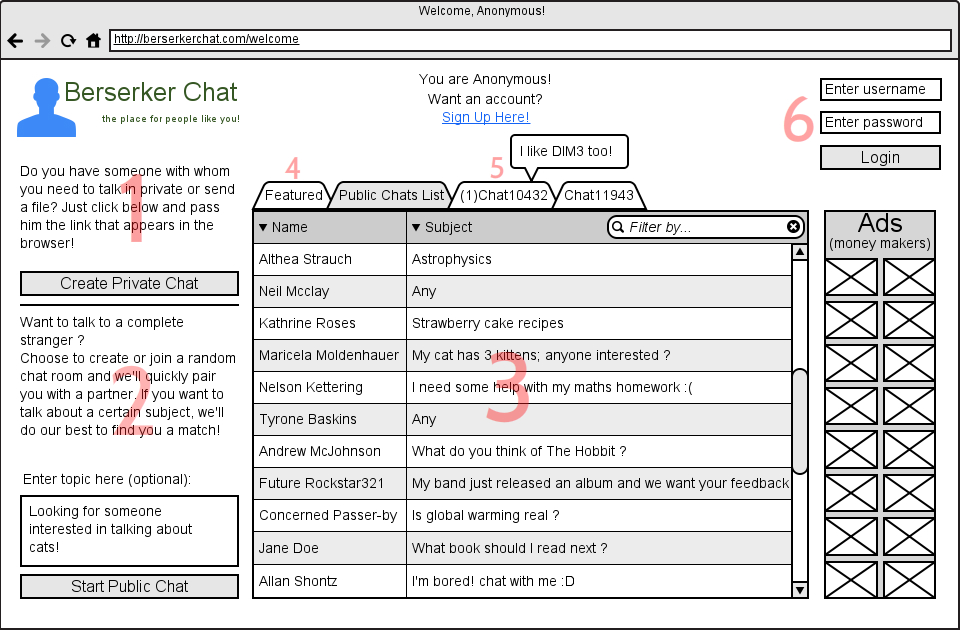
\includegraphics[scale=0.25]{wireframe_num.jpg}

\begin{enumerate}
\item This allows the user to create a private chat. When the `create private chat' button is clicked, a link appears in the browser which the user can click to redirect them to the correct chat room. The private chat link can be passed to others: only those with the link can chat in that specific chat room. 
\item This allows the user to start a public chat. When the `start public chat' button is clicked the user is redirected to a random public chat room. If the user specifies a topic, then the user is redirected to a room for that topic, if it exists. If it does not exist, the room for the topic is created and the user can invite others to join, or wait for other people with the same interest to join.
\item This shows the list of public chats and the name of the person who started it. Clicking on a particular chat subject takes the user into that chatroom. 
\item The featured tab shows the chats which have had the most users and are therefore very popular. This allows the user to see what the main topics of chat are.
\item A tab shows the chats the user is currently participating in with a pop-up of the most recently received message.
\item Allows the user to login and logout of the site
\end{enumerate}

%include screenshots of the real thing and compare and contrast. Basically the real thing is quite close to the wireframe but some things have been simplified for example we can only go down on level in the categories and not two. Also categories and most recent/popular has been introduced.

\begin{itemize}
%\item	Draw a wireframe of the user interface %include the png of the main screen from moqups
\item	this may require several wireframes depending on the complexity of the application and the interfaces %include 3 screenshots from the main thing
\item	Describe the user interface. 
\item	i.e. Label key input and output components: describe them.
\item	Provide a Walkthrough and explain the user interactions with application. %walkthrough of starting a public chat for a particular topic, finding a particular topic and starting a chat
\item	i.e. use cases
\item	Describe the interactions associated with the dynamic components on the user interface. %the chat messages are dynamically updated.
\item	What calls are required to dynamically update the data on the client side?
\item	How does the user interface help the user achieve their goal, or complete their task? 
\item	Is the user interface intuitive, appealing, usable, etc?
\item	What technologies are used on the client side? %HTML CSS JS
\item	What are the reasons for your choices? i.e. what is the advantages and disadvantages of using this technology? %popular web technologies supported by all main browsers
\item	What other options are there? %HTML5 %Responsive CSS framework such as Bootstrap, Zurb, Foundations
\end{itemize}

\section{Application Architecture}
The application is designed to use a 3-tier architecture as illustrated in the diagram below. Using this type of architecture allows
a separation of concerns between the display of the content on the client browser, the web application framework, and the backend.

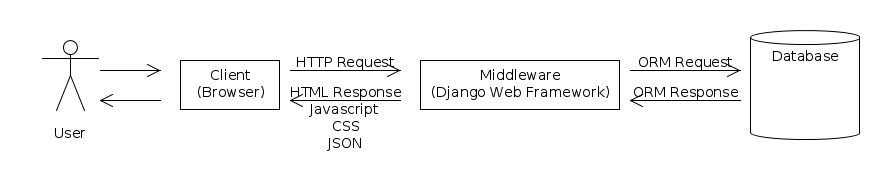
\includegraphics[scale=0.3]{n-tier-arch.png}
The 3-tier architecture consists of: \\\\ 
\textbf{Client} \\
The client (user) interacts with the Berserker Chat application through a web browser\\ \\
\textbf{Middleware} \\
The middleware is where the Django web framework is positioned. It essentially glues together the client and the backend, providing views based on data contained within the database and also updating the database based on the interactions of the user at the browser interface level.\\ \\
\textbf{Database} \\
The database stores information about the models which can be requested by the middleware by an Object Relational Model request. The database is implemented using SQLite3.\\ \\

\begin{itemize}
\item	N-Tier Architecture Diagram %nearly done
\item	i.e. data flow diagram between the interface/client, middle ware, and backend services/data repos %nearly done
\item	Describe the data model i.e. what data needs to be stored or persisted by the application? %todo
\item	What are the relationships within the data model. %todo
\item	i.e. use ER diagram and explain. %todo
\item	Describe the backend services used (if any). %sqlite3 db to store...
\item	Reflective Questions: 
\item	How have you ensured that there is a separation of concerns? %used the mvc pattern equivalent of django: model view template MTV 
\item	What other technology could have been used instead of django? %php web frameworks: cakewalk, symphony. others: ruby on rails, spring 
\item	What are the advantages of using a Web Application Framework over other technology? %more structure perhaps over php for example; encourages a separation of concerns 
\item	And, what are the disadvantages? %development time could be longer if one is to maintain a clear structure. some web apps can be put together in a short space of time but violate the fundamental separation of concerns that is promoted by the Django web application framework
\end{itemize}

\subsection{Reflections on Application Architecture}
Separation of concerns is extremely important to ensure a consistent structure of the application and to ensure maintainability. It also allows development to happen in parallel, e.g. someone could be working on the HTML and CSS of a page, and someone could be working on the database backend. The separation of concerns in this application has been achieved by using the Model, View, Template pattern in Django. \\

This allows the display of the application on the user's browser to be separated from the business logic of the application. The view is responsible for mapping a URL to the data which should be displayed. The template controls how the data identified by a particular view is displayed to the user. The model is essentially a description or definition of the data that the application stores in a database. This maps easily to a relational database model. The view interacts with the model to obtain information for display using the template. \\

Other web technologies/frameworks could have been used instead of Django with some gaining a lot of traction and support from the web development community. Some of these are: Symphony, Ruby on Rails and Cakewalk. \\

\textbf{Advantages and Disavantages of using Web Application Frameworks (WAFs)}
\begin{itemize}
\item Web application frameworks can decrease the time it takes to develop an application but also introduces the possibiity of a high learning curve to learn how to effectively and efficiently use the framework to enhance web development.
\item Many WAFs are built upon some underlying design patterns, e.g. Django effectively uses the Model-View-Controller (MVC) pattern. This encourages the developer to adhere to software engineering best practices, which in turn allows high quality, maintanable applications to be built.
\item Security issues and bugs found in the framework can affect all application that use that particular framework.
\end{itemize}

\section{Message Parsing}
\subsection{Sending a chat message}
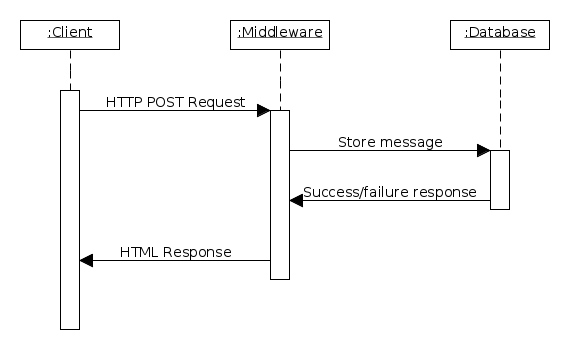
\includegraphics[scale=0.4]{postmessage.png}


\subsection{Displaying chat messages}
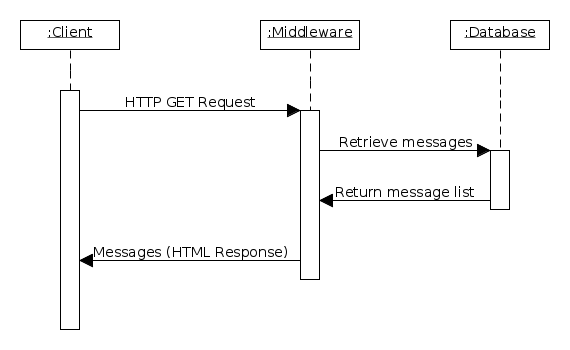
\includegraphics[scale=0.4]{getmessage.png}


\begin{itemize}

\item	On the architecture diagram, Identify and label the main messages that will be parsed through the application.
\item	or alternatively (and preferably) include sequence diagrams to denote the sequence of communications parse between clients and servers.
\item	Describe the messages that are parsed back and forth through the application.
\item	For the main transactions - describe the payload of the messages 
\item	i.e. What are the contents of the messages? i.e. include sample XML, XHTML, JSON, etc of one or two messages.
\item	What is the format of the messages? 
\item	Why this format? 
\item	What other formats could be used, what are the advantages and disadvantages of these other formats?
\end{itemize}


\section{Implementation Notes}
\label{sec: implementation}

\begin{itemize}
\item Views - What are the main views that you have implemented and what do they do?
\item URL Mapping Schema - what is your URL mapping and schema?
\item External Services  - what external services does your application include and what handlers did you include?
\item	Functionality Checklist (which functionality is completed)
\item	Known Issues (what kind of works, what kind of errors to do you get)
\item What technologies have been used and are required for the application. Include a list or table of all the technologies, standards, and protocols that will be required.
\end{itemize}

\section{Reflective Summary}
{\bf For the Implementation Report Only:}
\begin{itemize}
\item	What have you learnt through the process of development? 
\item	How did the application of frameworks help or hinder your progress? 
\item	What problems did you encounter? 
\item	What were your major achievements?
\end{itemize}

\section{Summary and Future Work}
\begin{itemize}
\item	Summary of application and its current state.
\item	Include a list or table of all the technologies, standards, and protocols that will be required.
\item	What are the limitations?
\item Plans for future development
\end{itemize}

\section{Acknowledgements}
Our thanks to the lecturers and demonstrators for their comments and suggestions. And our thanks to the peer reviewers for their feedback.
Be sincere and be specific about how others have helped your group.


\bibliographystyle{abbrv}
\bibliography{sig-proc}

\end{document}
